% Класс документа пока не окончательный, сильно сомневаюсь, что article 		
\documentclass[a4paper,12pt]{extarticle} 
% Подключаем шрифты,кодировки,русские переносы
\usepackage{cmap}
% подключается пакет, позволяющий улучшить вид пдф документа(как я понял)
\usepackage[utf8x]{inputenc}
% подключаем кодировку шрифтов для вносимых файлов
\usepackage[T2A]{fontenc}
% подключаем кодировку внутреннних шрифтов
\usepackage[main=russian,english]{babel}
% подключаем перенос и распознование слов, русский в приоритете
\usepackage{indentfirst}
% Отступ в начале абзаца
% \usepackage[unicode=true,pdfusetitle,
 	% bookmarks=true,bookmarksnumbered=false,bookmarksopen=true,
 	% breaklinks=false,pdfborder={0 0 0},pdfborderstyle={},backref=slide,colorlinks=false]
 	% {hyperref}
 % Надо разобраться с опциями, копирнул из пред.файла, который еще был написан в lyx
\usepackage{subfig}
% попытка загрузить minipage
\usepackage{
	amssymb,
	amsfonts,
	amsmath,
}
\usepackage{nicefrac}
% Пакеты американского математ. сообщества, красивый вид формул и текста внутри, а также дробный вид формул
\usepackage{esdiff}
% Пакет для производных
\usepackage{
	wrapfig,
	graphicx,
	caption,
	% subcaption,
	tikz,
}
\captionsetup{format=plain,labelsep=period}
% Обтекаемые объекты, рисунки, подписи без двоеточий и прочее
\usepackage{
	pgfplotstable,
	pgfplots,
	booktabs,
	colortbl,
	array,
	% float
}
\pgfplotsset{compat=newest}
% таблицы, графики
\usepackage[final]{pdfpages}
% Для вставки pdf файлов
\usepackage{geometry}
\usepackage{fancyhdr}
% границы, контитулы, и прочее


\geometry
	{
	left=1.5cm,
	right=1.5cm,
	bottom=2cm,
	top=2cm,
	}
% границы документа

\usepackage{setspace}
% убирает гигантские размеры оглавления
\linespread{1.3}
% междустрочный интервал

\pagestyle{fancy}
\fancyhead{}
% пустая шапка контитула
\fancyhead[R]{\authors}
% На правой стороне страницы авторы и науч.рук.
\fancyhead[L]{\labname}
 % Слева название лабы
\fancyfoot{}
\fancyfoot[C]{\thepage}
% номер страницы снизу по середине
\renewcommand{\contentsname}{Оглавление}
% переводим на русский язык оглавление
\usepackage{secdot}
\sectiondot{subsection}
% Ставит злосчастные точки в главах, ибо не по госту
% Преамбула почти слизана у Федора Сарафанова https://github.com/FedorSarafanov/RLC/blob/master/text/diss.tex

\usepackage{xcolor}
\usepackage{float}
\usepackage{hyperref}
\usepackage{tikz}
\usepackage{pgfplots}
\hypersetup{unicode=true}
\definecolor{linkcolor}{HTML}{799B03} % цвет ссылок
\definecolor{urlcolor}{HTML}{799B03} % цвет гиперссылок
 
\hypersetup{pdfstartview=FitH,  linkcolor=linkcolor,urlcolor=urlcolor, colorlinks=true}
\begin{document}
\sloppy
	\def\authors{Есюнин М.В., Есюнин Д.В.}
	\def\labnum{1}
	\def\labname{Многозвенные LC-фильтры}
	\def\sciadviser{Половинкин А.В.}
% \renewcommand{\contentsname}{Оглавление}
% \renewcommand{\figurename}{Рис.}
\renewcommand{\vec}{\mathbf}
\renewcommand{\phi}{\varphi}
\renewcommand{\kappa}{\varkappa}
% нормальный вид вектора, фи и каппа
\renewcommand{\Re}{\operatorname{Re}}
\renewcommand{\Im}{\operatorname{Im}}
% меняем номрмальное начертание Re and Im
\begin{titlepage}

\begin{center}

{\small\textsc{Нижегородский государственный университет имени Н.\,И. Лобачевского}}
\vskip 1pt \hrule \vskip 3pt
{\small\textsc{Радиофизический факультет}}

\vfill

{\Large Отчет по лабораторной работе №\labnumber\vskip 12pt\bfseries \labtheme}
	
\end{center}

\vfill
	
\begin{flushright}
	{Выполнили студенты \labgroup\ группы\\ \labauthors}%\vskip 12pt Принял:\\ Менсов С.\,Н.}
\end{flushright}
	
\vfill
	
\begin{center}
	Нижний Новгород, \the\year
\end{center}

\end{titlepage}


\begin{spacing}{1.2}
\tableofcontents
\end{spacing}
\numberwithin{equation}{section}
\newpage
\section{Уравнения многозвенного электрического фильтра}

Система, состоящая из цепочки идентичных звеньев, будучи системой с пространственной дисперсией, обладает селективными свойствами в определенной области частот. В зависимости от того, какова область частот, в которой колебания пропускаются практически без искажений, фильтры подразделяются на фильтры низких и высоких частот, полосовые и задерживающие фильтры.
\begin{figure}[h!]
	\centering
	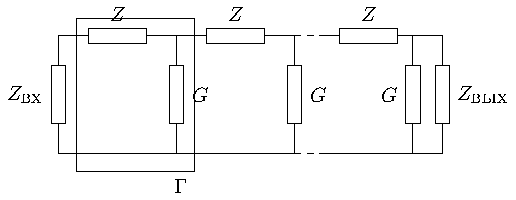
\includegraphics[]{picture1.pdf}
	\caption{Общая схема фильтра}
	\label{fig:1}
\end{figure}
Четырехполюсники, образующие звенья рассматриваемых в работе электрических фильтров, состоят из пассивных элементов: индуктивностей, ёмкостей и сопротивлений. Для большей методической простоты мы будем изучать только консервативные фильтры, состоящие из чисто реактивных элементов – индуктивностей и ёмкостей, так называемые LC - фильтры. Общая схема фильтра приведена на рис. \ref{fig:1}, где введены следующие обозначения:  $Z(p)$ – 
операторный импеданс,   $G(p)$ –операторная проводимость,   и  $Z_{\text{вх}}(p)$ и $Z_{\text{вых}}(p)$ – операторные импедансы на входе и выходе фильтра, соответственно, где $\omega$ – частота колебаний. При расчетах фильтры могут быть разбиты на так называемые Г-образные, Т- образные и П-образные звенья. Заметим, что такое деление -- чисто условное и не влияет на коэффициент передачи рассчитываемого фильтра.
% \begin{figure}[H]
% 	\centering
% 	\includegraphics[]{ris/ris.jpg}
% 	\caption{Общая схема фильтра}
% 	\label{fig:figure1}
% \end{figure}

Рассмотрим для примера фильтр, разбитый на Т-образные звенья (см. рис. \ref{fig:2}), и запишем для него операторные уравнения квазистатики.

\begin{figure}[h!]
	\centering
	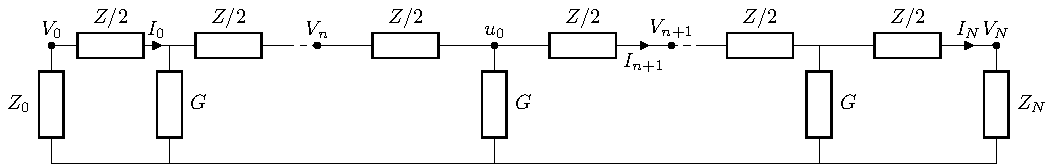
\includegraphics[]{picture2.pdf}
	\caption{Фильтр из Т-образных звеньев}
	\label{fig:2}
\end{figure}

При этом на основании законов Кирхгофа для комплексных амплитуд напряжений $V_n$ и токов $I_n$, где $n$ номер звена, будем иметь:
\begin{equation}
	\label{eq:1.1}
	\begin{gathered}
	V_n-U_0=\frac{Z}{2}I_n, \\
	U_0-V_{n+1}=\frac{Z}{2}I_{n+1}, \\
	GU_0=I_n-I_{n+1}
	\end{gathered}
\end{equation}
Исключая из этих уравнений $U_0$ и разрешая их относительно переменных $V_{n+1}$ и $I_{n+1}$, получим:
\begin{equation}
	\label{eq:1.2}
	\begin{gathered}
	V_{n+1}=a_{11}(p)V_n-a_{12}{p}I_n, \\
	I_{n+1}=-a_{21}V_n+a_{22}(p)I_n,
	\end{gathered}
\end{equation}
где
\begin{equation}
	\label{eq:1.3}
	\begin{gathered}
		a_{11}=1+\frac{1}{2}GZ,\; 
		a_{12}=Z\left(1+\frac{1}{4}GZ\right)\\
		a_{21}=G,\;
		a_{22}=1+\frac{1}{2}GZ
		\end{gathered}
\end{equation}

Отметим следующее важное свойство четырёхполюсников. Четырёхполюсники, для которых выполняются условия
\begin{equation}
	\label{eq:1.4}
	\begin{gathered}
		a_{11}=a_{22},\; 
		a_{12}=Z
	\end{gathered}
\end{equation}
называются взаимными.Для них выполняется теорема взаимности, согласно которой свойства четырёхполюсника не изменяются, если его вход и выход поменять местами. Нетрудно видеть, что Т-образное звено представляет собой взаимный четырёхполюсник. В случае П-образного разбиения на звенья в уравнениях \eqref{eq:1.2} следует положить 
\begin{equation}
	\label{eq:1.5}
	\begin{gathered}
		a_{11}=1+\frac{1}{2}GZ,\; 
		a_{12}=Z\\
		a_{21}=G\left(1+\frac{1}{4}GZ\right)\;
		a_{22}=1+\frac{1}{2}GZ
	\end{gathered}
\end{equation}
Отсюда следует, что П-образное звено также удовлетворяет теореме взаимности. 
Система \eqref{eq:1.2} должна быть дополнена граничными условиями
\begin{equation}
	\label{eq:1.6}
	\begin{gathered}
		V_0=-I_0Z_0,\; 
		V_N=Z_NI_N
	\end{gathered}
\end{equation}
Исследование явлений, описываемых уравнениями \eqref{eq:1.2} при условии \eqref{eq:1.6} включает в себя задачи:
\begin{enumerate}
	\item описание собственных колебаний
	\item описание вынужденных колебаний
\end{enumerate}
Прежде чем переходить к решению первой задачи, исследуем собственные колебания \eqref{eq:1.2} в безграничной цепочке, положим $N\rightarrow\infty$.

\section{Дисперсионное уравнение}
Важнейшей особенностью рассматриваемой цепочной структуры является её периодичность, являющаяся следствием идентичности звеньев и проявляющаяся при $N\rightarrow\infty$ в виде свойства так называемой \textit{трансляционной симметрии}. Это свойство равнозначно свойству инвариантности уравнений (\ref{eq:2.1}) относительно преобразования трансляции $n\Rightarrow n'$ вида $n'=n+m$, где m-- любое целое число. Трансляционная симметрия \eqref{eq:1.1} в сочетании с линейностью этих уравнений позволяет искать их решение в виде
\begin{equation}
\label{eq:2.1}
V_n=Ae^{-in\theta}, I_n=Be^{-in\theta},
\end{equation}
где $n=0,\pm1,\pm2,\dots,$, а $\theta$-- некоторая величина, подлежащая определению. Она находится из условия существования нетривиального решения алгебраической системы
\begin{equation}
	\label{eq:2.2}
	\begin{gathered}
	A(e^{-i\theta}-a_{11})+Ba_{12}=0, \\
	Aa_{21}+B(e^{-i\theta}-a_{22})=0,
	\end{gathered}
\end{equation}
получаемой подстановкой \eqref{eq:2.1} в \eqref{eq:2.2}. Этим условием является равенство нулю детерминанта \eqref{eq:2.2},что, с учётом \eqref{eq:1.4}, даёт
\begin{equation}
\label{eq:2.3}
(e^{-i\theta}-a_{11})^2-a^2_{11}+1=0
\end{equation}
или
\begin{equation}
\label{eq:2.4}
\cos\theta=a_{11}
\end{equation}

Величина $\theta$, определяемая из \ref{eq:2.4} называется \textit{постоянной распространения} и принимает в общем случае комплексные значения ($\theta=\theta'+i\theta''$).
Мнимая часть $\theta$ представляет собой декремент (или инкремент) волны, а действительная часть -- набег фазы волны на одно звено. При этом $\theta'$ связана с длиной волны $\lambda$ очевидным соотношением
\begin{equation}
\label{eq:2.5}
\lambda=2 \frac{\pi}{\theta'},
\end{equation}
в котором 
\begin{equation}
\label{eq:2.6}
\lambda=min|n_1-n_2|
\end{equation}
где и $n_1$ и $n_2$- номера ячеек, отвечающих синфазным колебаниям. Поскольку параметр является функцией частоты $\omega$, уравнение \eqref{eq:2.4} связывает постоянную распространения с частотой и называется дисперсионным уравнением системы. Дисперсионное уравнение исчерпывающе характеризует безграничную систему. В случае, когда отсутствует временное и пространственное затухание ($\Im\omega=\Im\theta=0$), оно позволяет определить фазовую ($V_{\text{ф}}$) и групповую ($V_{\text{гр}}$) скорости волн:
\begin{equation}
	\label{eq:2.7}
	\begin{gathered}
	V_{\textmd{ф}}=\frac{\omega}{\theta},\;
	V_{\text{гр}}=\frac{d\omega}{d\theta}
	\end{gathered}
\end{equation}
\begin{equation*}
(-\pi \leq\theta\leq\pi)	
\end{equation*}

Дисперсионное уравнение \eqref{eq:2.4} описывает два типа волн -- прямую ($\theta=\theta^+$) и обратную ($\theta=\theta^-$) волну. При этом для фиксированного $\omega$ значения $\theta^+ $и $\theta^-$ будут отличаться только знаком:
\begin{equation}
\label{eq:2.8}
\theta^-=-\theta^+.
\end{equation}
Подставляя $\theta^-$ и $\theta^+$ в одно из уравнений системы \eqref{eq:2.2}, можно найти связь между амплитудами напряжения и тока для прямой и обратной волн
\begin{equation}
\label{eq:2.9}
B^+=G_xA^+, B^-=-G_xA^-,
\end{equation}
где
\begin{equation}
\label{eq:2.10}
G_x=\left(\frac{a_{21}}{a_{12}}\right)^{\frac{1}{2}}
\end{equation}
--\textit{характеристическая проводимость фильтра}. Наряду с $G_x$, вводят также и обратную ей величину
\begin{equation}
\label{eq:2.11}
Z_x=\sqrt{\frac{a_{12}}{a_{21}}},
\end{equation}
именуемую \textit{характеристическим импедансом} фильтра.

Пространственная дисперсия фильтра (описываемая \ref{eq:2.4}) обуславливает его селективные свойства. Для характеристики этих свойств вводят понятие \textit{полосы прозрачности}, а именно полосы частот, в которой $\theta''=0$(отсутствует затухание по переменной n).

Найдём связь ширины полосы прозрачности с параметрами фильтра. С этой целью заметим, что поскольку
\begin{equation}
\label{eq:2.12}
\sin\theta=\ch\theta''\sin\theta'+i\sh\theta''\cos\theta',
\end{equation}
то в полосе прозрачности
\begin{equation}
\label{eq:2.13}
\sin\theta=\sin\theta'.
\end{equation}
Отсюда, в силу \eqref{eq:2.3}, заключаем, что
\begin{equation}
\label{eq:2.14}
1-a_{11}^2\geq 0,
\end{equation}
или, с учётом \eqref{eq:2.3},--
\begin{equation}
\label{eq:2.15}
GZ(1+\frac{1}{4}GZ)\leq 0
\end{equation}
Из этого условия и находится полоса прозрачности фильтра. Из него, в частности следует, что в полосе прозрачности фильтра характеристический импеданс \eqref{eq:2.11} будет действительной величиной.

Вне полосы прозрачности $\sin\theta'=0$ и, следовательно, $\sin\theta=i\sh\theta''$. С учётом \eqref{eq:3.4}, будем иметь
\begin{equation}
\label{eq:2.16}
\sh\theta''=\pm\sqrt{a_{11}^2-1}
\end{equation}

\section{Собственные колебания}
Найдём собственные колебания в цепочке, состоящей из N одинаковых Т-образных звеньев, описываемой системой уравнений \eqref{eq:2.2} при граничных условиях \eqref{eq:1.6}. Общее решение такой системы будет представлять собой суперпозицию прямой и обратной волн вида
\begin{equation}
	\label{eq:3.1}
	\begin{gathered}
	V_n=A_1e^{-i\theta}+A_2e^{i\theta}, \\
	I_n=B_1e^{-i\theta}+B_2e^{i\theta}.
	\end{gathered}
\end{equation}

Для внутренних звеньев прямая и обратная волны распространяются независимо и для них, в силу \eqref{eq:2.9}, общее решение запишется в виде
\begin{equation}
	\label{eq:3.2}
	\begin{gathered}
	V_n=A_1e^{-i\theta}+A_2e^{i\theta}, \\
	I_n=G_x(A_1e^{-i\theta}+A_2e^{i\theta}).
	\end{gathered}
\end{equation}
Подставляя это решение в граничные условия \eqref{eq:1.6},
получим следующую однородную систему уравнений для нахождения амплитуд $A_1$ и $A_2$:
\begin{equation}
	\label{eq:3.3}
	\begin{gathered}
	(1+Z_0G_x)A_1+(1-Z_0G_x)A_2=0,
	(1-Z_NG_x)e^{-iN\theta}A_1+(1+Z_NG_x)e^{iN\theta}A_2=0.
	\end{gathered}
\end{equation}

Отсюда, расписав условие существования ненулевых решений для $A_1$ и $A_2$, найдём \textit{характеристическое уравнение} рассматриваемой системы
\begin{equation}
\label{eq:3.4}
1-\Gamma_0\Gamma_Ne^{-2iN\theta}=0,
\end{equation}
где
$\displaystyle\Gamma_0\frac{A_1}{A_2}=-\frac{1-Z_0G_x}{1+Z_0G_x}$
--коэффициент отражения от левой границы фильтра, а
$\displaystyle\Gamma_N\frac{A_2e^{iN\theta}}{A_1e^{-iN\theta}}=
-\frac{1-Z_NG_x}{1+Z_NG_x}$
--коэффициент отражения от правой границы фильтра.

Решая совместно дисперсионное уравнение \eqref{eq:2.4} и характеристическое уравнение \eqref{eq:3.4}, найдём спектр собственных (нормальных) частот фильтра и соответствующий ему спектр значений постоянной распространения $\theta$. Очевидно, что этот спектр будет зависеть не только от параметров звена фильтра, но и от условий на его концах. Отметим также, что число нормальных частот всегда совпадает с числом степеней свободы системы.
\section{Вынужденные колебания}
Рассмотрим вынужденные колебания в фильтре, составленном из Т-образных звеньев, при условии, что на входе фильтра действует источник синусоидальной ЭДС $E=E_0\cos(\omega t)$ с внутренним сопротивлением $r_0$ (см. \ref{fig:3}). Решение в такой системе можно искать в виде синусоидальных колебаний на частоте внешней силы $\omega$. При этом остаются справедливыми уравнения \eqref{eq:1.2}, а граничные условия принимают вид:
\begin{equation}
	\label{eq:4.1}
	V_0=E_0-r_0Z_0,\;V_N=Z_NI_N.
\end{equation}
\begin{figure}[h!]
	\centering
	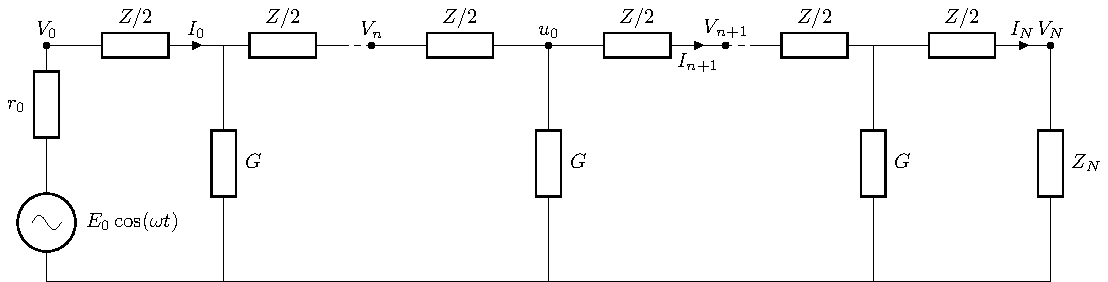
\includegraphics[]{picture3.pdf}
	\caption{}
	\label{fig:3}
\end{figure}
Подставляя \eqref{eq:3.2} в \eqref{eq:4.1}, получим 
\begin{equation}
	\label{eq:4.2}
	\begin{gathered}
	(1+r_0G_x)A_1+(1-r_0G_x)A_2=E_0\\
	(1-Z_NG_x)e^{-iN\theta}A_1+(1+Z_NG_x)e^{iN\theta}A_2=0
	\end{gathered}
\end{equation}
Отсюда для $A_1$ и $A_2$ будем иметь
\begin{equation}
	\label{eq:4.3}
	\begin{gathered}
	A_1=\frac{1-\Gamma_0}{2}\cdot\frac{E_0}{1-\Gamma_0\Gamma_Ne^{-2iN\theta}},\\
	A_2=\frac{1-\Gamma_0}{2}\cdot\frac{E_0\Gamma_Ne^{-2iN\theta}}{1-\Gamma_0\Gamma_Ne^{-2iN\theta}},\\
	\end{gathered}
\end{equation}
Подставляя \eqref{eq:4.3} в \eqref{eq:3.2}, получим следующие выражения для комплексных амплитуд напряжения $V_n$ и $I_n$ тока в n-ой ячейке:
\begin{equation}
	\label{eq:4.4}
	\begin{gathered}
	V_n=\frac{1-\Gamma_0}{2}\cdot\frac{E_0e{-in\theta}}{1-\Gamma_0\Gamma_Ne^{-2iN\theta}}\left[1+\Gamma_Ne^{-2i(N-n)\theta}\right],\\
	I_n=\frac{1-\Gamma_0}{2}\cdot\frac{E_0e{-in\theta}}{1-\Gamma_0\Gamma_Ne^{-2iN\theta}}G_x\left[1-\Gamma_Ne^{-2i(N-n)\theta}\right],\\
	\end{gathered}
\end{equation}
Из \eqref{eq:4.4} следует, что если частота внешней ЭДС совпадает с одной из собственных частот фильтра, то амплитуды напряжений и токов во всех звеньях фильтра принимают бесконечно большие значения (явление резонанса). Очевидно, что это возможно лишь в отсутствии затухания, т. е. при условии $\Im\omega_m=0$. В реальных системах всегда существуют потери ($\omega_m=\omega'_m+i\omega''_m$) и знаменатель в \eqref{eq:4.4} не обращается в ноль. При этом в случае произвольных потерь картина резонанса достаточно сложна и далека от той, какую мы имеем в одиночном резонансном контуре. Однако, при $\omega''_m/\omega'_m<<1$ эта картина существенно упрощается, и влияние потерь можно описать на привычном языке добротности, вводя её для каждой моды отношением
\begin{equation}
\label{eq:4.5}
Q_m=\omega'_m/\omega''_m
\end{equation}
Таким образом, для системы со многими степенями свободы не имеет смысла говорить о добротности системы вообще, необходимо оговаривать, о добротности какой моды идёт речь.

При изучении вынужденных колебаний важную роль играют два семейства статических характеристик: семейство амплитудно-частотных характеристик (АЧХ) и семейство фазо-частотных характеристик (ФЧХ). Эти семейства находятся из выражения для коэффициента передачи, представляющего собой отношение комплексной амплитуды напряжения на выходе фильтра к амплитуде ЭДС на входе, т.е.
\begin{equation}
\label{eq:4.6}
W(\omega)=\frac{V_N(\omega)}{E_0(\omega)}=\frac{(1-\Gamma_0)(1+\Gamma_N)e^{-iN\theta}}{2\left(1-\Gamma_0\Gamma_Ne^{-2iN\theta}\right)}
\end{equation}
По определению АЧХ -- это функция 
\begin{equation}
\label{eq:4.7}
A(\omega)=|W(\omega)|
\end{equation}
а ФЧХ -- функция
\begin{equation}
\label{eq:4.8}
\Phi(\omega)=-argW(\omega)
\end{equation}
Очевидно, что вид того и другого семейства характеристик зависит от условий на концах фильтра.

Рассмотрим влияние этих условий на $A(\omega)$ и $W(\omega)$ в полосе прозрачности фильтра, полагая для простоты, что нагрузка фильтра чисто активная (т. е. $\Gamma_0$ и $\Gamma_N$ –действительные функции). При этом
\begin{equation}
\label{eq:4.9}
A(\omega)=\frac{1-\Gamma_0}{2}\cdot\frac{1+\Gamma_N}
{\sqrt{1-\Gamma_0\Gamma_N\cos2N\theta+\Gamma^2_0\Gamma^2_N}}
\end{equation}
Из полученного выражения следует, что если фильтр согласован на обоих концах ($\Gamma_0=\Gamma_N=0$), то $A(\omega)=1/2$, т.е. напряжение источника ЭДС делится поровну между фильтром и внутренним сопротивлением источника. Если фильтр согласован только на входе ($\Gamma_0=0$), или только на выходе($\Gamma_N=0$), то $A(\omega)=(1+\Gamma_N)/2$ и $A(\omega)=(1-\Gamma_0)/2$, соответственно. Во всех трёх случаях АЧХ не зависит от числа звеньев фильтра.
 
Если фильтр согласован хотя бы на одном из своих концов, а нагрузка на другом конце -- чисто активная, то существенно упрощается и $\Phi(\omega)$:
\begin{equation}
\label{eq:4.10}
\Phi(\omega)=N\theta(\omega)
\end{equation}
Т.е. ФЧХ с точностью до множителя N сводится к дисперсионной характеристике фильтра.

Многозвенные фильтры представляют собой разновидность длинных линий и используются в радиотехнических устройствах в качестве \textit{линий задержки}. Время запаздывания сигнала при прохождении его через фильтр легко оценить для случая узкополосного сигнала при условии, что спектр его лежит в полосе прозрачности фильтра и укладывается в диапазон частот, в котором фазо-частотную характеристику фильтра можно считать линейной. Спектральную плотность такого сигнала на выходе фильтра для прямой волны можно записать в виде
\begin{equation}
\label{eq:4.11}
u_N(\eta)=A_1(\xi)e^{i[(\Omega+\eta)t-N\theta(\Omega+\eta)t]}
\end{equation}
Учитывая, что $|\eta|\leq\Delta\omega$, где $\Delta\omega$ -- полуширина спектра, и принимая во внимание условие узкополосности $\Delta\omega<<\Omega$, разложим в этом выражении нелинейную функцию $\theta(\Omega+\eta)$ в ряд по степеням $\eta$, ограничившись двумя первыми членами:
\begin{equation}
\label{eq:4.12}
\theta(\Omega+\eta)\approx\theta(\Omega)+\left.\frac{d\theta}{d\omega}\right|_\Omega \eta
\end{equation}
При этом выражение \eqref{eq:4.11} примет вид
\begin{equation}
\label{eq:4.13}
u_N(\eta)\approx A_1(\xi)e^{i[\Omega t-N\theta\Omega]}e^{i(t-N\frac{d\theta}{d\omega}\eta)}
\end{equation}
Отсюда следует, что время задержки сигнала при прохождении через N-звенный фильтр равно $\tau_N=N\frac{d\omega}{d\theta} \Omega$. Т.е. групповая скорость $(d\omega\ /d\theta)$ имеет смысл времени запаздывания, приходящегося на одно звено.
\section{Фильтр низкой частоты (ФНЧ)}
Вид отдельного звена ФНЧ изображен на рис \ref{fig:1.1}. ФНЧ служит для пропускания колебаний низкой частоты от $\omega=0$ до $\omega_{\text{ср}}$ (\textit{частота "среза"}). Для ФНЧ
\begin{equation}
\label{eq:5.1.1}
Z=i\omega L,\;G=i\omega C.
\end{equation}
\begin{figure}[h!]
	\begin{minipage}{0.49\linewidth}
		\centering
		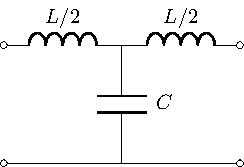
\includegraphics[]{FLF/FLFT.pdf}
		\caption*{Т-образное звено}
	\end{minipage}
\begin{minipage}{0.49\linewidth}
	\centering
	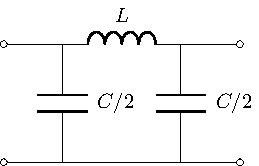
\includegraphics[]{FLF/FLFP.pdf}
	\caption*{П-образное звено}
\end{minipage}
\caption{}
\label{fig:1.1}
\end{figure}
При этом \textbf{диспресионное уравнение} имеет вид 
\begin{equation}
\label{eq:5.1.2}
\omega^2=\frac{2}{LC}(1-\cos\theta)
\end{equation}
\begin{figure}[h!] 
	\centering
	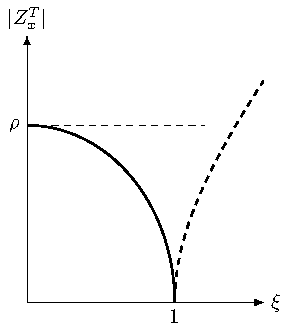
\includegraphics[]{FLF/ZxT.pdf}
	\caption{}
	\label{fig:1.2}
\end{figure}
Из периодического характера этого уравнения следует, что физический смысл имеет лишь та часть дисперсионных ветвей, которая лежит в области $|\theta|\leq\pi$. Т.е. набег фазы на одно звено не может превышать $\pi$. Поскольку постоянная распространения $\theta$ связана с длиной волны $\lambda$ соотношением $\lambda=2\pi/\theta$, то из существования $\theta_{\text{max}}=\pi$ вытекает существо-вание $\lambda_{\text{min}}$. Иными словами, волны с длиной в одну ячейку существовать не могут. Этот результат порождён дискретным характером структуры фильтра и может быть предсказан заранее.

\textbf{Полоса прозрачности} ФНЧ, в силу \eqref{eq:2.15}, задаётся условием
\begin{equation}
\label{eq:5.1.3}
\omega^2\leq\frac{4}{LC}\; (\xi^2=\frac{\omega^2}{\omega^2_{\text{ср}}}\leq1)
\end{equation}

\textbf{Характеристический импеданс} фильтра, состоящего из Т- и П-образных звеньев задаётся соотношениями
\begin{equation}
	Z^T_x=\rho\sqrt{1-\xi^2},\;
	Z^{\text{П}}_x=\frac{\rho}{\sqrt{1-\xi^2}},\;
	(\rho=\sqrt{L/C})
\end{equation}
\begin{figure}[h!]
\begin{minipage}{0.49\linewidth}
	\centering
	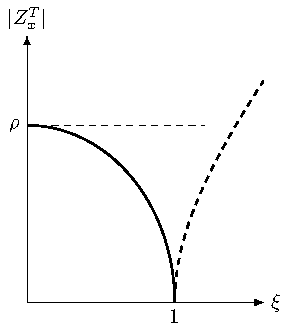
\includegraphics[]{FLF/ZxT.pdf}
\end{minipage}
\begin{minipage}{0.49\linewidth}
	\centering
	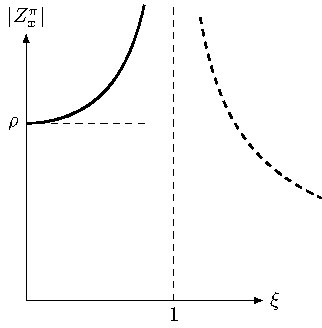
\includegraphics[]{FLF/ZxP.pdf}
\end{minipage}
\caption{}
\label{fig:1.3}
\end{figure}
Соответствующие им частотные зависимости изображены на рис. \ref{fig:1.3}.

\textbf{Параметры звеньев фильтра} рассчитываются по формулам
\begin{equation}
	\label{eq:5.5}
	L=\frac{2\rho}{\omega_{\text{ср}}},\;
	C=\frac{2}{\rho\omega_{\text{ср}}}
\end{equation}
Время задержки на одно звено даётся выражением
\begin{figure}[H]
	\centering
	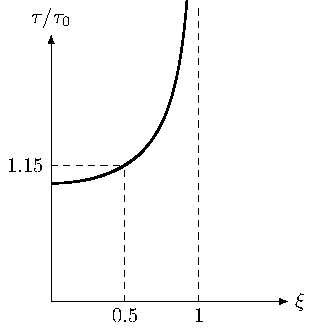
\includegraphics[]{FLF/tau1.pdf}
	\caption{}
	\label{fig:1.4}
\end{figure}
\begin{equation}
\label{eq:5.6}
\tau=\frac{2}{\omega_{\text{ср}}\sqrt{1-\xi^2}}
\end{equation}
Графически зависимость времени задержки от частоты изображена на рис. \ref{fig:1.4}
\section{Фильтр высокой частоты (ФВЧ)} 
Вид отдельного звена ФВЧ изображен на рис \ref{fig:6.1}. ФВЧ служит для пропускания колебаний с частотами $\omega\geq$. Для ФНЧ
\begin{equation}
\label{eq:6.1.1}
Z=i/\omega C,\;G=i/\omega L.
\end{equation}
\begin{figure}[h!]
	\begin{minipage}{0.49\linewidth}
		\centering
		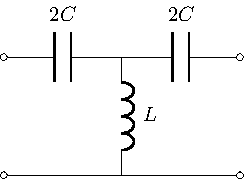
\includegraphics[]{FHF/FHFT.pdf}
		\caption*{Т-образное звено}
	\end{minipage}
	\begin{minipage}{0.49\linewidth}
		\centering
		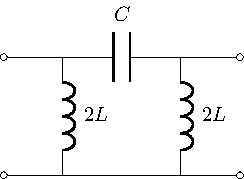
\includegraphics[]{FHF/FHFP.pdf}
		\caption*{П-образное звено}
	\end{minipage}
	\caption{}
	\label{fig:6.1}
\end{figure}
При этом \textbf{диспресионное уравнение} имеет вид 
\begin{equation}
\label{eq:6.1.2}
\omega^2=\frac{1}{2LC(1-\cos\theta)}
\end{equation}
График дисперсионной зависимости приведен на рис. \ref{fig:6.2}
\begin{figure}[h!]
	\centering 
	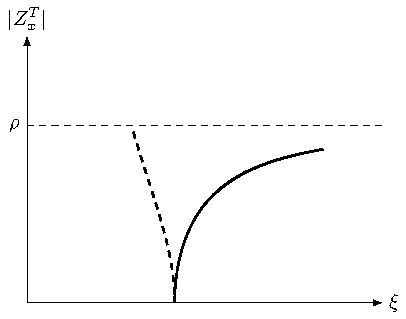
\includegraphics[]{FHF/ZxP2.pdf}
	\caption{}
	\label{fig:6.2}
\end{figure}


\textbf{Полоса прозрачности} ФНЧ, определяется из условия 
\begin{equation}
\label{eq:6.1.3}
1-\frac{1}{4\omega^2LC\geq0}\;(\xi^2\geq1)
\end{equation}

\textbf{Характеристический импеданс} фильтра, состоящего из Т- и П-образных звеньев задаётся соотношениями
\begin{equation}
Z^T_x=\rho\sqrt{1-\frac{1}{\xi^2}},\;
Z^{\text{П}}_x=\frac{\rho\xi}{\sqrt{\xi^2-1}},\;
(\rho=\sqrt{L/C})
\end{equation}
\begin{figure}[h!]
	\begin{minipage}{0.49\linewidth}
		\centering
		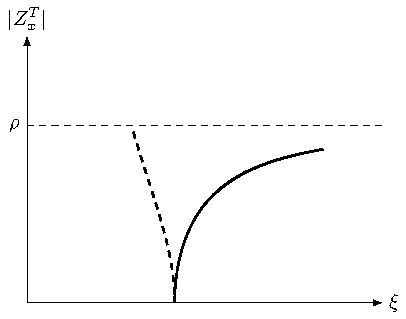
\includegraphics[]{FHF/ZxP2.pdf}
	\end{minipage}
	\begin{minipage}{0.49\linewidth}
		\centering
		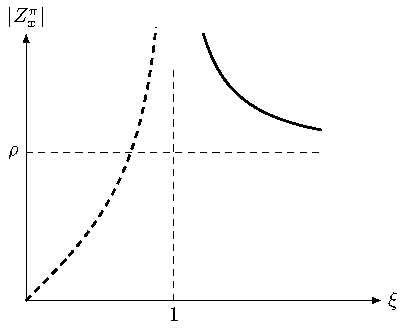
\includegraphics[]{FHF/ZxT2.pdf}
	\end{minipage}
	\caption{}
	\label{fig:6.3}
\end{figure}
Соответствующие им частотные зависимости изображены на рис. \ref{fig:6.3}.

\textbf{Параметры звеньев фильтра} рассчитываются по формулам
\begin{equation}
\label{eq:6.5}
L=\frac{\rho}{2\omega_{\text{ср}}},\;
C=\frac{1}{2\rho\omega_{\text{ср}}}
\end{equation}
Время задержки на одно звено даётся выражением
\begin{figure}[h!]
	\centering
	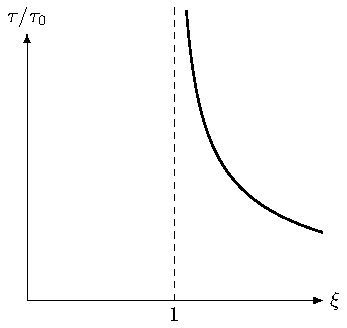
\includegraphics[]{FHF/tau2.pdf}
	\caption{}
	\label{fig:6.4}
\end{figure}
\begin{equation}
\label{eq:6.6}
\tau=\frac{1}{\omega_{\text{ср}}\xi\sqrt{\xi^2-1}}
\end{equation}
Графически зависимость времени задержки от частоты изображена на рис.\ref{fig:6.4}
\section{Полосовой фильтр}
Вид отдельного звена полосового фильтра изображен на рис.\ref{fig:7.1}. Полосовой фильтр служит для пропускания колебаний в полосе частот$\omega_1\leq\omega\leq\omega_2$.
\begin{figure}[h!]
	\begin{minipage}{0.49\linewidth}
		\centering
		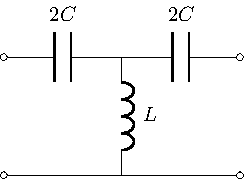
\includegraphics[]{FHF/FHFT.pdf}
		\caption*{Т-образное звено}
	\end{minipage}
	\begin{minipage}{0.49\linewidth}
		\centering
		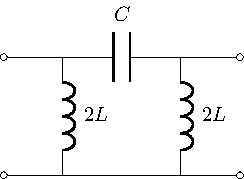
\includegraphics[]{FHF/FHFP.pdf}
		\caption*{П-образное звено}
	\end{minipage}
	\caption{}
	\label{fig:7.1}
\end{figure}
Для полосового фильтра
\begin{equation}
\label{eq:7.1}
Z=i\omega L_1+i/\omega C_1,\;G=i\omega C_2+i/\omega L_2.
\end{equation}
\textbf{Дисперсионное уравнение} полосового фильтра определяется следующей зависимостью
\begin{equation}
	\label{eq:7.2}
	f(\omega^2)=\sin^2\frac{\theta}{2}
\end{equation}
где
\begin{equation}
	\label{eq:7.3}
	f(\omega^2)=\frac{(L_1C_1\omega^2-1)(L_2C_2\omega^2-1)}{4\omega^2L_2C_1}
\end{equation}

\begin{figure}[h!]
	\centering 
	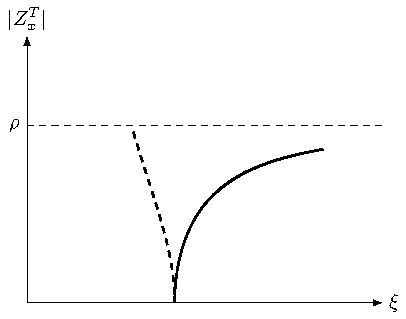
\includegraphics[]{FHF/ZxP2.pdf}
	\caption{}
	\label{fig:7.2}
\end{figure}
Так как $\displaystyle 0\leq\sin^2\frac{\theta}{2}\leq1$, то система будет пропускать частоты $\displaystyle\omega_1\leq\omega\leq\frac{1}{\sqrt{L_1C_1}}$ и $\displaystyle frac{1}{\sqrt{L_1C_1}}\leq\omega\leq\omega_2$. На практике интересен случай, когда $\displaystyle \frac{1}{\sqrt{L_1C_1}}=\frac{1}{\sqrt{L_2C_2}}=\omega_0$, $\displaystyle \frac{L_1}{L_2}=\frac{C_1}{C_2}=\alpha$
При этом дисперсионное уравнение принимает вид
\begin{equation}
\label{eq:7.4}
\left(\frac{\omega^2}{\omega^2_0}-1\right)\frac{\omega_0}{2\omega}\sqrt{\alpha}=\pm\sin\frac{\theta}{2}
\end{equation}
Соответствующие ему дисперсионные кривые изображены на рис.\ref{fig:7.3}
\begin{equation}
\label{eq:7.5}
\omega_1=\frac{\omega_0}{\sqrt{\alpha}}(\sqrt{1+\alpha}-1),\;
\omega_2=\frac{\omega_0}{\sqrt{\alpha}}(\sqrt{1+\alpha}+1)
\end{equation}
\begin{figure}
	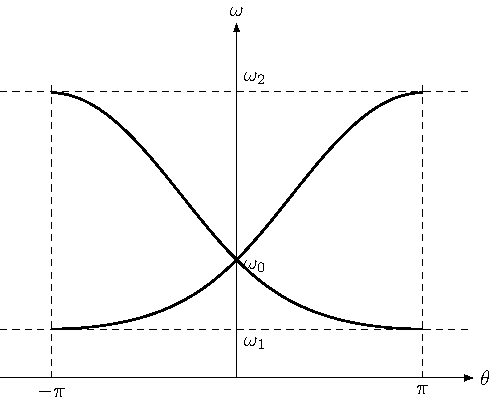
\includegraphics[]{FF/w(0).pdf}
	\caption{}
	\label{fig:7.3}
\end{figure}
\textbf{Полоса прозрачности} фильтра определяется из условия 
\begin{equation}
\label{eq:7.6}
\left(\frac{\omega}{\omega_0}-\frac{\omega_0}{\omega}\right)^2\alpha\leq 4.
\end{equation}
\textbf{Характеристический импеданс фильтра}, состоящего из Т- и П- образных звеньев соотношениями
\begin{equation}
\label{eq:7.7}
Z^T_x=\rho\sqrt{1-\frac{\alpha}{4}\left(\frac{\omega}{\omega_0}-\frac{\omega_0}{\omega}\right)^2},\;
Z^\text{П}_x=\frac{\rho}{\sqrt{1-\frac{\alpha}{4}\left(\frac{\omega}{\omega_0}-\frac{\omega_0}{\omega}\right)^2}}
\end{equation}
где $\rho=\sqrt{L_2/C_1}$. Зависимость этого импеданса от частоты приведена на рис.\ref{fig:7.4}
\begin{figure}
\begin{minipage}{0.49\linewidth}
	\centering
	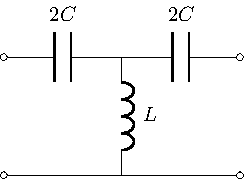
\includegraphics[]{FHF/FHFT.pdf}
\end{minipage}
\begin{minipage}{0.49\linewidth}
	\centering
	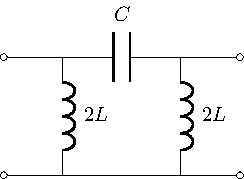
\includegraphics[]{FHF/FHFP.pdf}
\end{minipage}
\caption{}
\label{fig:7.4}
\end{figure}

\textbf{Параметры фильтра} рассчитываются по следующим формулам:
\begin{equation}
\label{eq:7.8}
\begin{gathered}
L_1=\frac{\sqrt{\alpha}\rho}{\omega_0}=\frac{2\rho}{\omega_2-\omega_1},\;
L_2=\frac{L_1}{\alpha}=\frac{\rho(\omega_2-\omega_1)}{2\omega^2_0}\\
C_1=\frac{1}{\omega^2_0L_1}=\frac{\omega_2-\omega_1}{2\rho\omega_1\omega_2},\;
C_2=\alpha C_1=\frac{2}{\rho(\omega_2-\omega_1)}\\
\rho=\sqrt{\frac{L_2}{C_1}}=\sqrt{\frac{L_1}{\alpha C_1}}
\end{gathered}
\end{equation}
\section{Эксперимент}
\subsection{ФЧХ и АЧХ}
% Собрали схему ФНЧ для 6 звеньев. Построили ФЧХ и АЧХ.
% \begin{minipage}{\linewidth}
% 	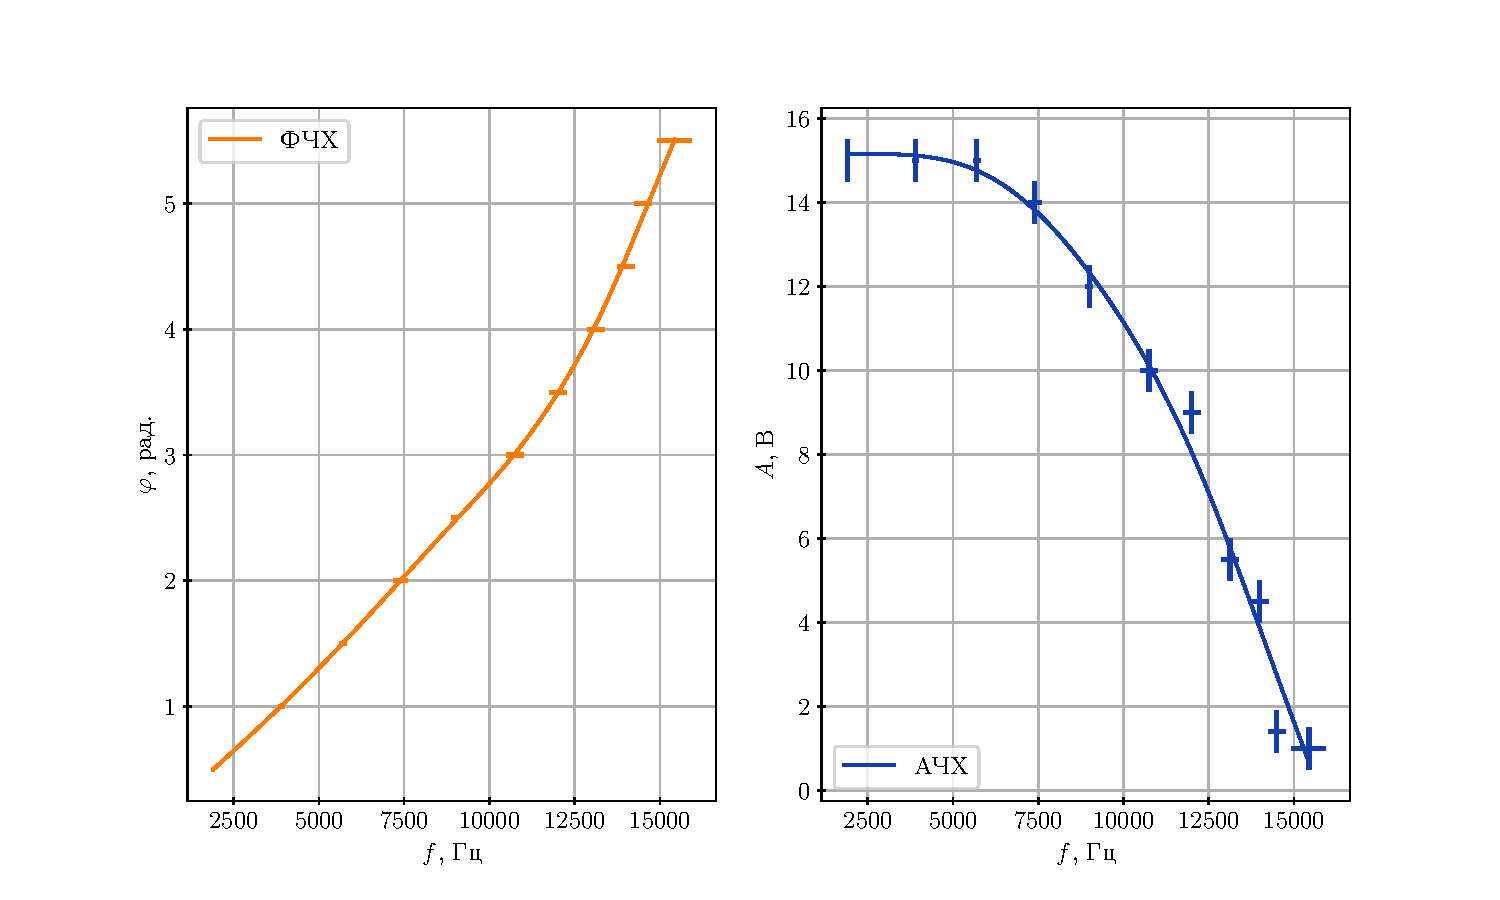
\includegraphics[width=\linewidth]{plots/FLF.pdf}
% 	\caption{}
% 	\label{exp:1}
% \end{minipage}

\end{document}
